\documentclass{article}\usepackage{graphicx, color}
%% maxwidth is the original width if it is less than linewidth
%% otherwise use linewidth (to make sure the graphics do not exceed the margin)
\makeatletter
\def\maxwidth{ %
  \ifdim\Gin@nat@width>\linewidth
    \linewidth
  \else
    \Gin@nat@width
  \fi
}
\makeatother

\definecolor{fgcolor}{rgb}{0.2, 0.2, 0.2}
\newcommand{\hlnumber}[1]{\textcolor[rgb]{0,0,0}{#1}}%
\newcommand{\hlfunctioncall}[1]{\textcolor[rgb]{0.501960784313725,0,0.329411764705882}{\textbf{#1}}}%
\newcommand{\hlstring}[1]{\textcolor[rgb]{0.6,0.6,1}{#1}}%
\newcommand{\hlkeyword}[1]{\textcolor[rgb]{0,0,0}{\textbf{#1}}}%
\newcommand{\hlargument}[1]{\textcolor[rgb]{0.690196078431373,0.250980392156863,0.0196078431372549}{#1}}%
\newcommand{\hlcomment}[1]{\textcolor[rgb]{0.180392156862745,0.6,0.341176470588235}{#1}}%
\newcommand{\hlroxygencomment}[1]{\textcolor[rgb]{0.43921568627451,0.47843137254902,0.701960784313725}{#1}}%
\newcommand{\hlformalargs}[1]{\textcolor[rgb]{0.690196078431373,0.250980392156863,0.0196078431372549}{#1}}%
\newcommand{\hleqformalargs}[1]{\textcolor[rgb]{0.690196078431373,0.250980392156863,0.0196078431372549}{#1}}%
\newcommand{\hlassignement}[1]{\textcolor[rgb]{0,0,0}{\textbf{#1}}}%
\newcommand{\hlpackage}[1]{\textcolor[rgb]{0.588235294117647,0.709803921568627,0.145098039215686}{#1}}%
\newcommand{\hlslot}[1]{\textit{#1}}%
\newcommand{\hlsymbol}[1]{\textcolor[rgb]{0,0,0}{#1}}%
\newcommand{\hlprompt}[1]{\textcolor[rgb]{0.2,0.2,0.2}{#1}}%

\usepackage{framed}
\makeatletter
\newenvironment{kframe}{%
 \def\at@end@of@kframe{}%
 \ifinner\ifhmode%
  \def\at@end@of@kframe{\end{minipage}}%
  \begin{minipage}{\columnwidth}%
 \fi\fi%
 \def\FrameCommand##1{\hskip\@totalleftmargin \hskip-\fboxsep
 \colorbox{shadecolor}{##1}\hskip-\fboxsep
     % There is no \\@totalrightmargin, so:
     \hskip-\linewidth \hskip-\@totalleftmargin \hskip\columnwidth}%
 \MakeFramed {\advance\hsize-\width
   \@totalleftmargin\z@ \linewidth\hsize
   \@setminipage}}%
 {\par\unskip\endMakeFramed%
 \at@end@of@kframe}
\makeatother

\definecolor{shadecolor}{rgb}{.97, .97, .97}
\definecolor{messagecolor}{rgb}{0, 0, 0}
\definecolor{warningcolor}{rgb}{1, 0, 1}
\definecolor{errorcolor}{rgb}{1, 0, 0}
\newenvironment{knitrout}{}{} % an empty environment to be redefined in TeX

\usepackage{alltt}
\IfFileExists{upquote.sty}{\usepackage{upquote}}{}

\begin{document}

\title{The randPort package}
\author{Mike Flynn, Angel Zhou, and Dave Kane}
\maketitle

\section*{Introduction}

Stuff about making random portfolios and why they are important.

\section*{Methodology}

\subsection*{getWeights}

getWeights takes equality constraints in the form of $$ E x = E
x_0$$ where $x_0$ is the weights of an original portfolio that we
desire to match. It also guarantees that all the output weights will
be positive. Starting from the original portfolio, we do a random walk
based in the null space of $E$. This guarantees that the equality
constraints will still hold via:$$ E(x_0 + v) = Ex_0 + Ev = Ex_0$$ if
$Ev = 0$ (the definition of a vector in the null space). To fully
sample the problem we have $v = Z*r$ where Z is a matrix whose columns
span the null space, and $r$ is a random vector whose coefficients
$r_i \sim N(0, 1)$. This can be interpreted geometrically as moving in
a random direction on the hyperplane that is the null-space. On each
step, getWeights checks if any of the weights are negative, if
they are, it projects the negative components onto the basis vectors
in $Z$ and subtracts those vectors from step. This guarantees that the
equality constraints will still hold, while none of the weights will
be less than zero.

\subsection*{Example}

Consider a universe with only 3 stocks, and our only constraint is
that their weights must add up to 1. Let our original portfolio be
represented by the vector $x_0 = (.3, .3, .4)$. Our equality matrix $E$
can be represented by the one-row matrix $E = [1,1,1]$. All our
solutions are necessarily in the plane $x + y + z = 1$. To check if
getWeights does this, we can look at a scatterplot of the
results.

\begin{knitrout}
\definecolor{shadecolor}{rgb}{0.969, 0.969, 0.969}\color{fgcolor}\begin{kframe}
\begin{alltt}
\hlfunctioncall{library}(scatterplot3d)
E = \hlfunctioncall{matrix}(\hlfunctioncall{c}(1, 1, 1), 1, 3)
x0 = \hlfunctioncall{c}(0.3, 0.3, 0.4)
w = \hlfunctioncall{getWeights}(E, x0, 1000)
\hlfunctioncall{scatterplot3d}(x = w[1, ], y = w[2, ], z = w[3, ], angle = 160)
\end{alltt}
\end{kframe}
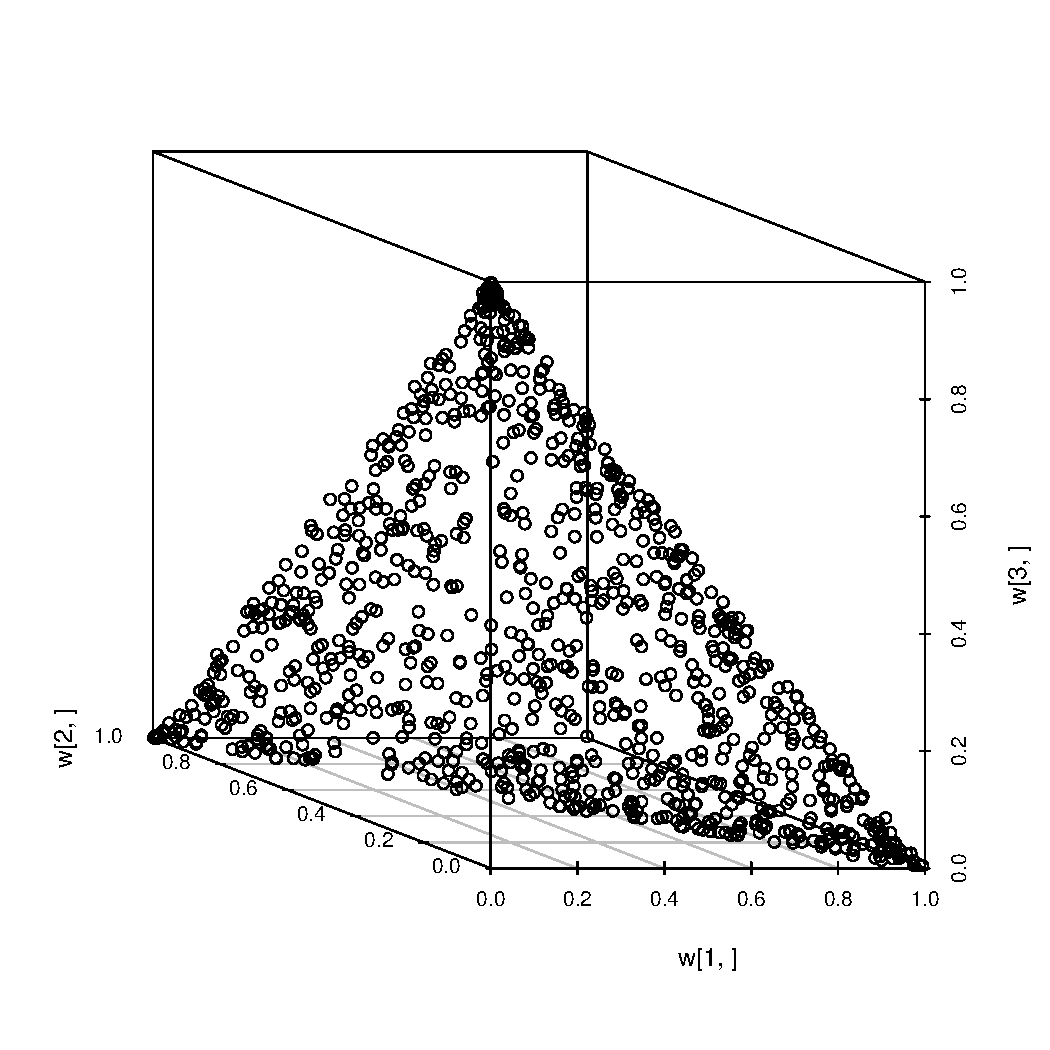
\includegraphics[width=\maxwidth]{figure/rcodeblockyeah} 

\end{knitrout}


Adding an additional constraint effectively reduces the dimensionality
of the solution space by 1, because if $E$ has one more row, the null
space will have one less column. In our example, $Z$ will only have on
vector, so we will essentially be stepping back and forth in one
direction on the surface. Demonstrating:

\begin{knitrout}
\definecolor{shadecolor}{rgb}{0.969, 0.969, 0.969}\color{fgcolor}\begin{kframe}
\begin{alltt}
E = \hlfunctioncall{rbind}(E, \hlfunctioncall{rnorm}(3))
\hlcomment{## x0 can be the same}
w = \hlfunctioncall{getWeights}(E, x0, 1000)
\hlfunctioncall{scatterplot3d}(x = w[1, ], y = w[2, ], z = w[3, ], angle = 160)
\end{alltt}
\end{kframe}
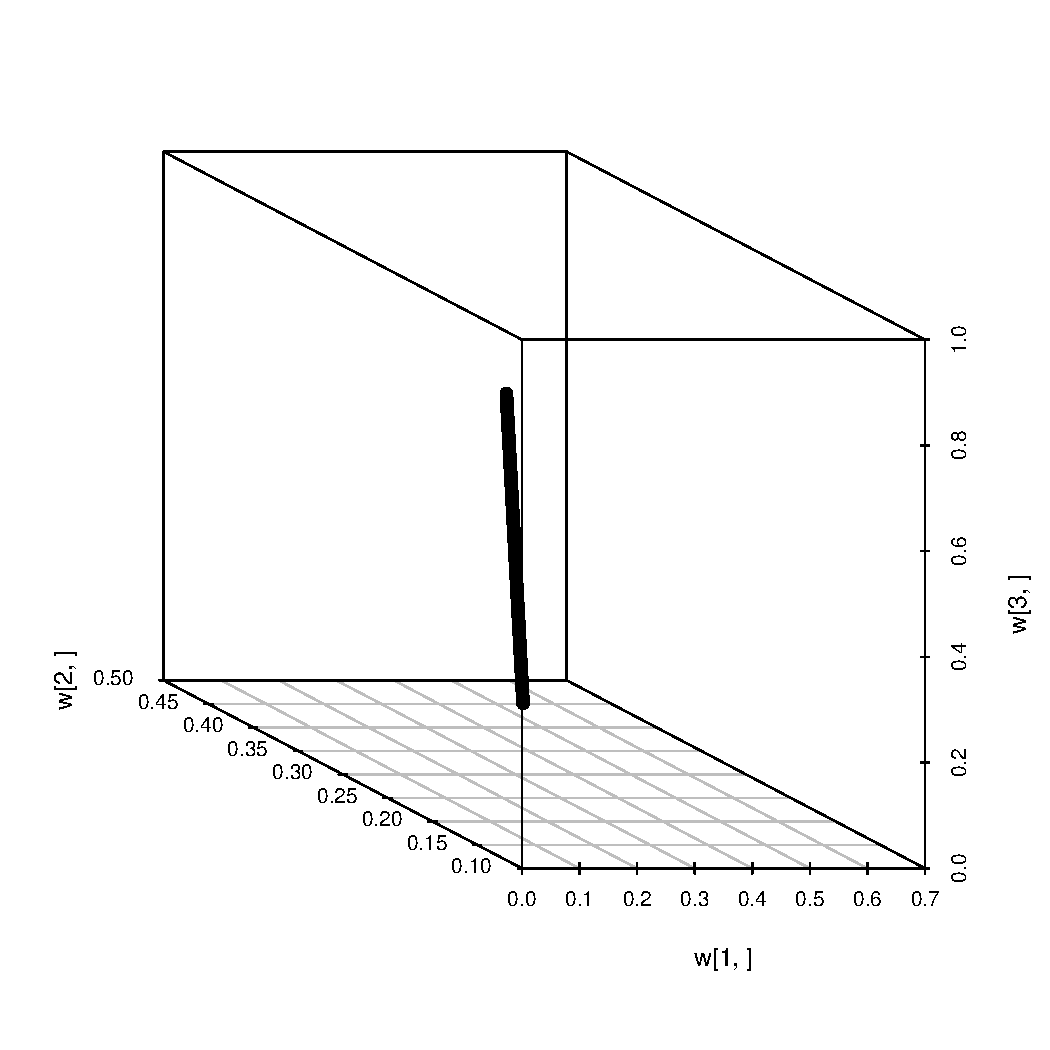
\includegraphics[width=\maxwidth]{figure/demo} 

\end{knitrout}


\end{document}
